\documentclass[reprint,english,notitlepage]{revtex4-2}
\usepackage{amsmath}
\usepackage[mathletters]{ucs}
\usepackage[utf8x]{inputenc}
\usepackage[english]{babel}
\usepackage{esint}
\usepackage{physics,amssymb}
\usepackage{graphicx}
\usepackage{xcolor}
\usepackage{hyperref}
\usepackage{listings}
\usepackage{subfigure}
\hypersetup{
    colorlinks,
    linkcolor={red!50!black},
    citecolor={blue!50!black},
    urlcolor={blue!80!black}}

\lstset{inputpath=,
    backgroundcolor=\color{white!88!black},
    basicstyle={\ttfamily\scriptsize},
    commentstyle=\color{magenta},
    language=Python,
    morekeywords={True, False},
    tabsize=4,
    stringstyle=\color{green!55!black},
    frame=single,
    keywordstyle=\color{blue},
    showstringspaces=false,
    columns=fullflexible,
    keepspaces=true}

\begin{document}

\title{Special Relativity}
\author{Candidates: 15369 \& 15401}
\date{\today}
\affiliation{Institute of Theoretical Astrophysics, University of Oslo}


\maketitle

\section{Exercise 1}\label{ex: 1}

  \subsection{Introduction}
  In this part we are going to explore the consequences of light traveling at a constant velocity in all frames of reference. The effect of this will give us some insight in how this we perceive the order of which events take place in different frames of reference. This is key to understanding how Einstein derived Special Relativity. We will do this by looking at two different reference points and only using the equation for position $ r = r_0 + vt + \frac{1}{2} at ^{2} $. 

  \subsection{The Situation}
  In this situation we have two spaceships traveling at the same constant speed with a distance $ L $ in between them. In the middle there is an observer $ M $ traveling at the same speed as the spaceships. We will look at two different frames of reference. One is the frame of reference of a planet below the spaceships. Here, time and space is denoted by $ t $ and $ x $ respectively. We also have the frame of reference of the observer $ M $ where time and space is denoted by $ t' $ and $ x' $ respectively. 
  
  We also have four events happening. Event A is the left most spaceship shooting its laser towards the right most ship. This occurs at $  x = x' = 0 $ and $ t = t' = 0 $. Event B is the right most ship shooting its laser towards the left most ship. Event C is when the left most ship is hit by the laser from the right most ship. Event D is when the right most ship is hit by the left most ship. 
  
  \colorbox{red}{Legg til bilder av event A og B events} 

  \subsection{Method}
  We will begin by exploring these events from the perspective of the observer $ M $. 
  Let's begin at event A and B. From the observer's point of view it, as well as the spaceships, are standing still. Both spaceships shoot their lasers at the same time (event A and B). How will the observer in the middle perceive this? Quite predicatively and maybe intuitively you would expect the observer to observe these events happening simultaneously. This is a natural conclusion as both beams of light are shot at the same time and have to travel the same distance $ L / 2 $. 
  
  Now let's explore this at this from the planets' perspective using only the following we know from the perspective of the observer.
  
  \begin{enumerate}
    \item The observer sees two light beams cross its position at the same time
    \item The observer is in the middle of the two spaceships 
    \item From the observer's perspective the lasers were shot out at the same time
  \end{enumerate}
  
  We know the first point to be true, as light travels at a constant velocity $ c $ in all frames of references, the light from both lasers must reach the observer on the planet at the same time if they are at the same location.
  From the planet reference we can calculate the time it takes each laser to reach the spacecraft in the middle by. Just solving the equation for position of each laser equal to the position of the observer $ M $ with respect to time, we get one expression of the time the lasers used to reach the observer $ M $ as derived in \ref{o: 1.1.2}. 
  \begin{equation}\label{eq: t_L}
    t_L = \frac{L /2}{1 - v}
  \end{equation}
  \begin{equation}\label{eq: t_R}
    t_R = \frac{L / 2}{1 + v}
  \end{equation}
  
  
  For event C and D we expect the same result as event A and B when seeing this from the perspective of observer $ M $. Both lasers will again travel with the same speed to reach the spaceships spaced equally far apart and stationary. 
  From the planet's perspective we must again do some calculations. As we derive in \ref{o: 1.1.4}, the time it takes the beam to travel from the observer $ M $ to the left most ship and right most ship is the following.
  \begin{equation}\label{eq: t_C}
    t_C = \frac{L / 2}{1 + v}
  \end{equation}
  \begin{equation}\label{eq: t_D}
    t_D = \frac{L / 2}{1 - v}
  \end{equation}
  
  
  
  
  
  \subsection{Conclusion} 
  From the perspective of the observer $ M $ we get the result of both beams being shot at the same time and arriving at the observer at the same time as well. When looking at it from the perspective of the planet the result are quite surprising if you have no knowledge of special relativity. As seen in equations \ref{eq: t_L} and \ref{eq: t_R} we notice the laser from the left most ship takes a longer time to reach the observer $ M $ than the laser from the right most ship. This is not surprising as you can imagine the lasers from the left most ship "chasing" after the observer and the observer running towards the laser from the right most ship. The only solution to this incongruence is that the laser were in fact not shot out at the same time! To reach the same place at the same time the laser from the left most ship must have been shot out before the laser from the right most ship. 
  
  This carries over to the explosion of each ship (event C and D). As derived in equations \ref{eq: t_C} and \ref{eq: t_D}. We must conclude the same as before. From the perspective of the planet, event C must happen before event D. 
  
  In conclusion, when looking at the events from the perspective of the planet, event A must happen before event B. Event C must happen before event D. As event A and B must both happen before they can cross observer $ M $, we also know both happen before event C and D. This gives the following chain of events. \\
  A → B → C → D.\\
  
  In \ref{1.2.1} we have calculated the time it takes for the beams to reach the observer and the time the beam shot from the right most ship uses to reach the left most spaceship. This was all done using the planet as the reference point. After that we looked at the same calculations from the perspective of the observer M. In this perspective we noticed a different time being calculated. In the eyes of the observer M it took a shorter time for the left most ship to shoot its own laser beam before being shot.
  The ratio of this time period denoted by $ Δt $ and $ Δt' $ corresponding to the planet's and observer's respective references were the following.
  \[
  \frac{Δt'}{Δt} = 1 - v^{2}
  \]
  As $ v $ is a fraction of the speed of light, the ratio of $ Δt' $ and $ Δt $ is below 1. If we rearrange the expression above we get the familiar 
  \[
  Δt = \frac{Δt'}{1 - v^{2}}
  \]
  This is very close to the actual formula for time dilation. 
  \[
  Δt = \frac{Δt'}{\sqrt{1 - v^{2}} }
  \]
  We are just missing a factor of $ \sqrt{1 - v^{2}}  $! This is also known as $ γ^{-1} $ where $ γ $ is the Lorentz factor. In special relativity there is not only a difference in time between reference points, but also distance.


\section{Exercise 4}

  \subsection{Introduction}
  In this exercise we are going to explore the concept of worldlines in a space-time diagram. This is a graph that plots movement along one axis with respect to time. We will also look at how different frames of reference change how these graphs look. An example of this kind of graph can be seen in figure \ref{fig: WL Example}. Here we see three different paths from event A to B. Notice the right most line having a tangent line with a slope lower than $ 45^{∘} $ at the very beginning. This would actually be impossible as it would mean whatever traveling would have a velocity higher than the speed of light. The line in the middle showcases a constant velocity. The left most line showcases some acceleration and deceleration during its journey. 
  
  As we already learned from the previous exercise \ref{ex: 1}, time moves differently in different frames of reference. We will explore this some more in the reference frame of the space station in comparison to spaceship 3
  
  
  \begin{figure}[h!]
    \centering
    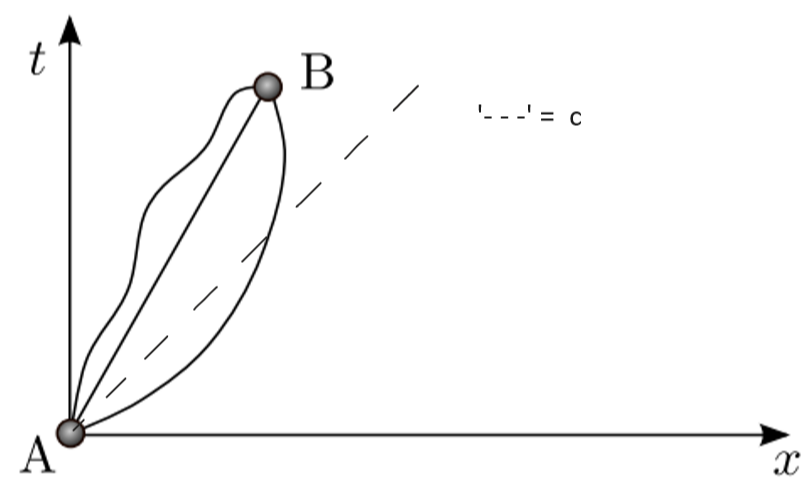
\includegraphics[scale = .5]{figures/worldline_example.png}
    \caption{Example of three different worldlines connecting two events A and B in time and space. Source: \ref{ref: Example worldline}}
    \label{fig: WL Example}
  \end{figure}
  
  \subsection{The Situation}
  The situation at hand is three spaceships (1: yellow, 2: red, 3: green) and one space station starting at the same position at the same time as seen in figure \ref{fig: Initial position}. We will explore the worldlines from the perspective of ship 1, 2 and the space station, which will be referred to as 4. From the perspective of the space station we will perceive spaceship 1 and 2 to travel with constant velocity, while spaceship 3 will both accelerate and decelerate. Naturally the space station will be stationary in its own frame of reference. This is also true for all ships. 
  \begin{figure}[h!]
    \centering
    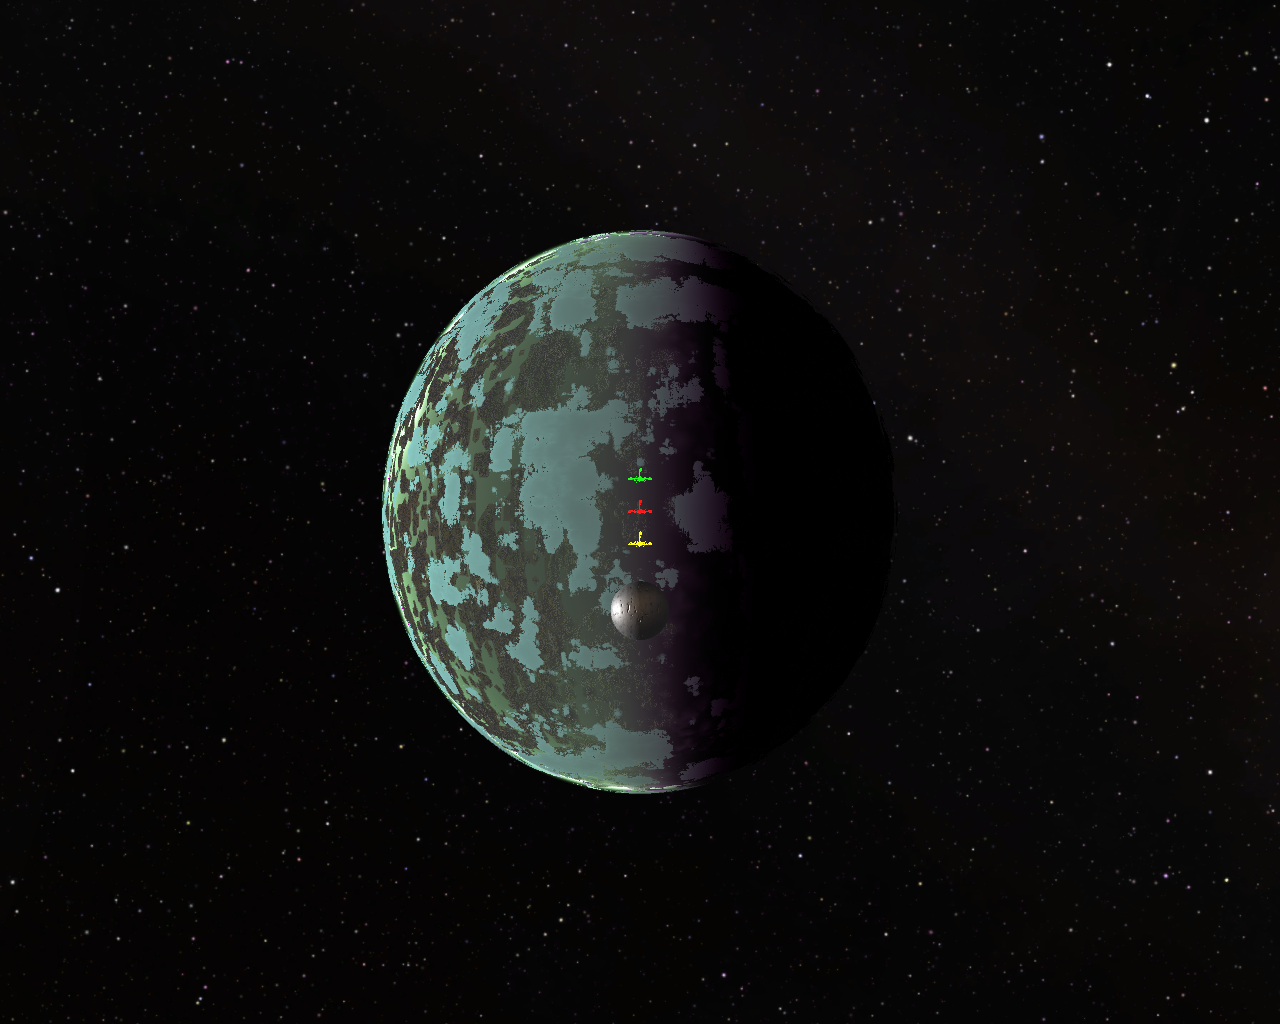
\includegraphics[scale = .125]{figures/Spaceships_t_0.png}
    \caption{Initial positions of space station and ships.}
    \label{fig: Initial position}
  \end{figure}
  
  \begin{figure}[h!]
    \centering
    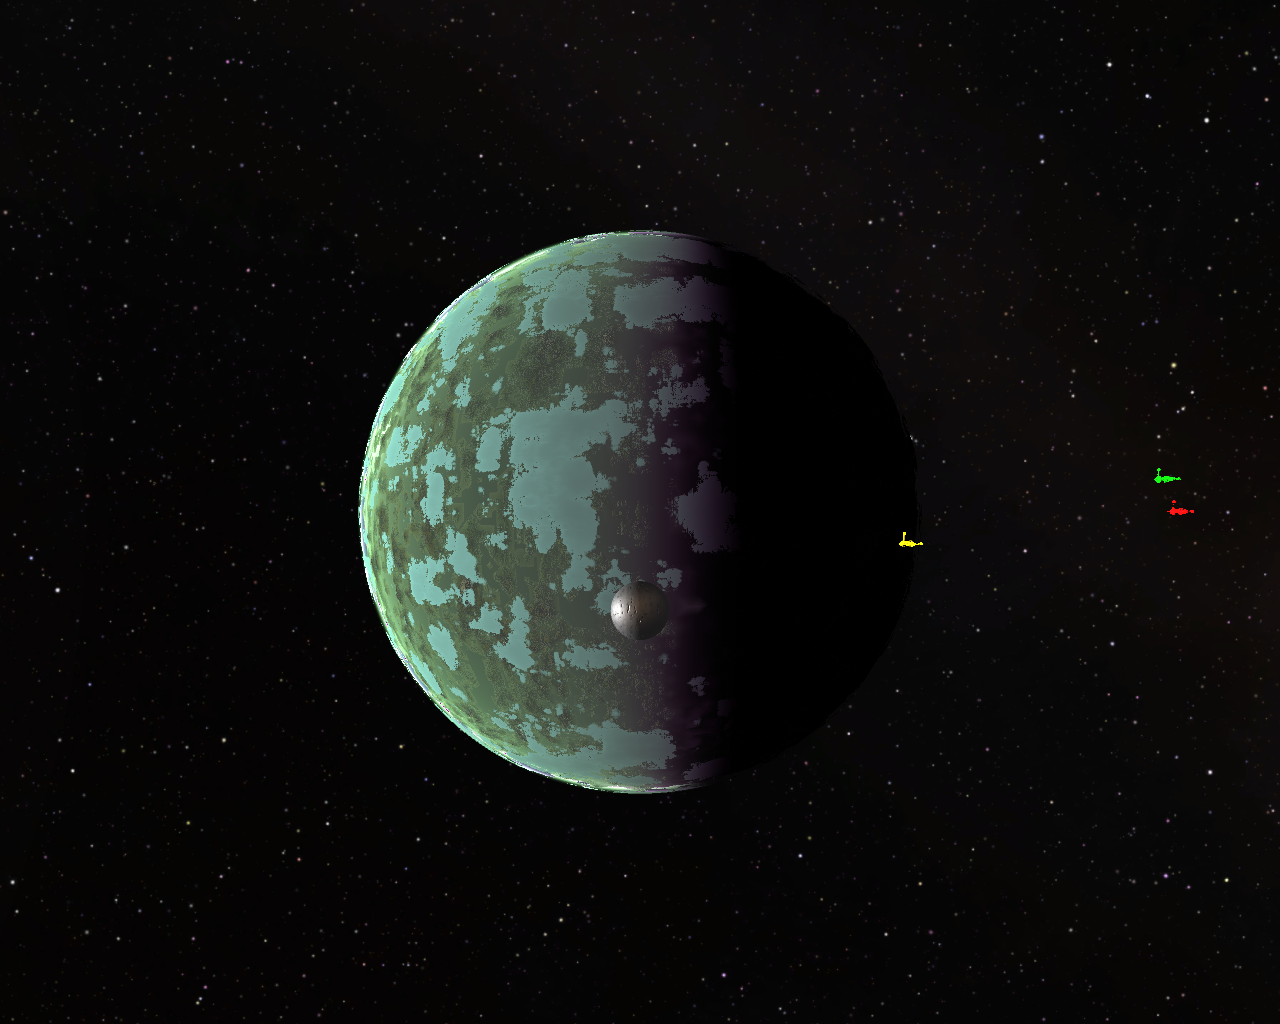
\includegraphics[scale = .125]{figures/Station_perspective.png}
    \caption{The system as seen from the perspective of the space station}
    \label{fig: Situation Station}
  \end{figure}
  \begin{figure}[h!]
    \centering
    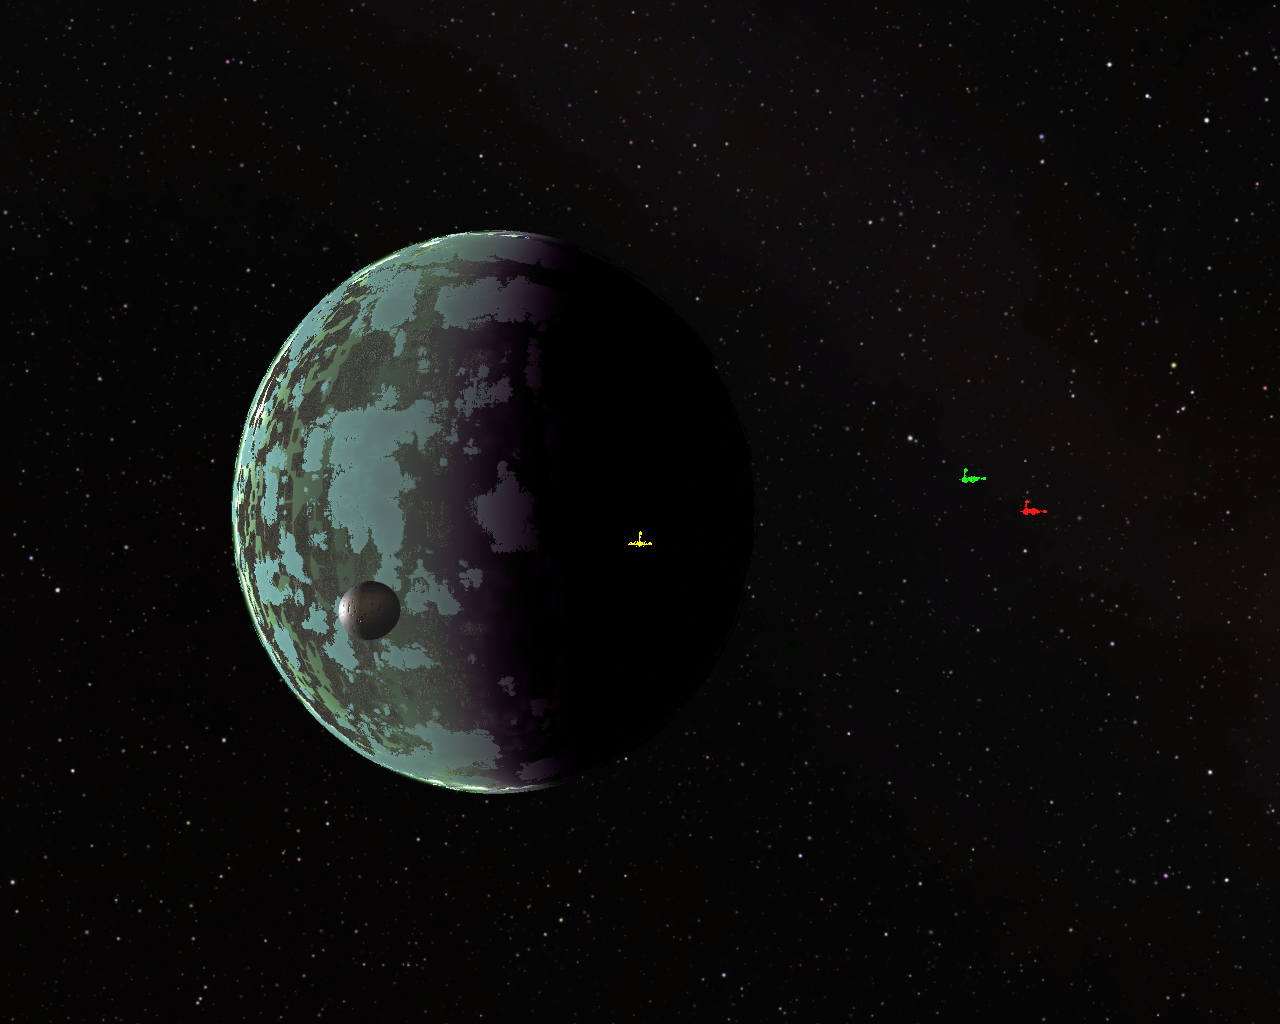
\includegraphics[scale = .125]{figures/1_perspective.png}
    \caption{The system as seen from the perspective of ship 1}
    \label{fig: Situation 1}
  \end{figure}
  \begin{figure}[h!]
    \centering
    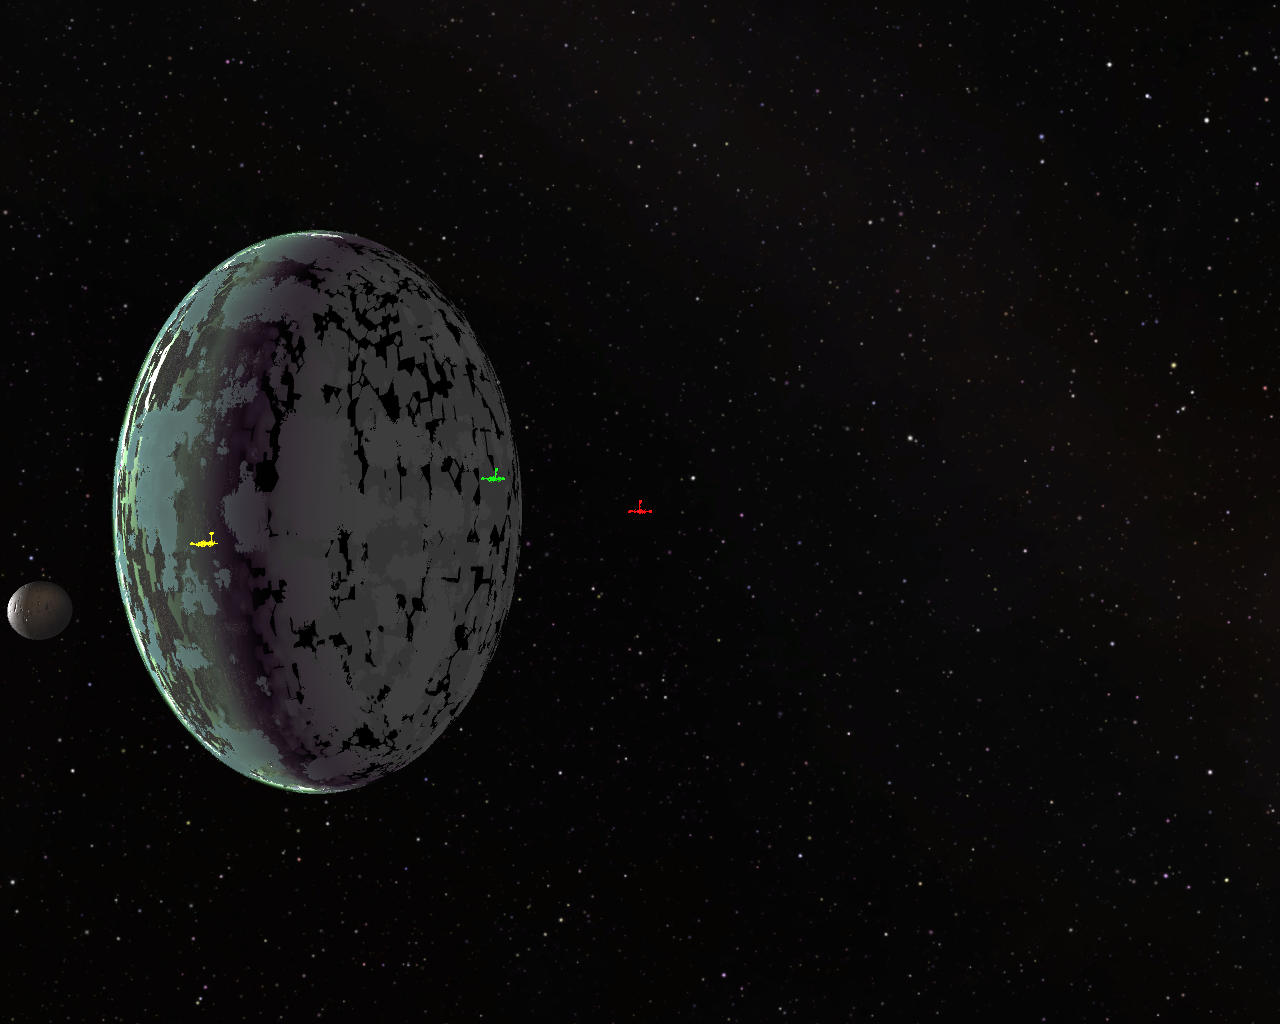
\includegraphics[scale = .125]{figures/2_perspective.png}
    \caption{The system as seen from the perspective of ship 2}
    \label{fig: Situation 2}
  \end{figure}
  
  When looking at the difference of time measured by the different observers we will define two event. Event 1 is defined as where $ t = 0 $ and all ships are in the same position as seen in \ref{fig: Initial position}. Event 2 is when spaceship 3 catches up to spaceship 2. The spaceship measures this taking 10 miliseseconds, while the clock on spaceship 2 measures 8 miliseconds. 

  \subsection{Method}
  To draw the worldlines we will look at the movement of each ship to get a rough estimate of their velocities in relation to one another. If two objects are at the same place at the same time we expect their worldlines to intersect.

  We will begin by looking at the worldlines from the perspective \ref{fig: Situation Station} of the space station. As mentioned before, it itself will be stationary and will perceive spaceship 1 and 2 to will have constant velocity while 3 will accelerate and decelerate. The time-space diagram will then be as seen in figure \ref{fig: Perspective Station}
  \begin{figure}[h!]
    \centering
    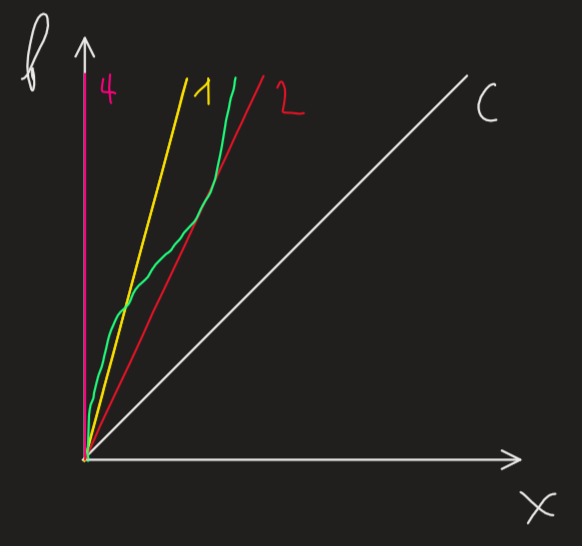
\includegraphics[scale = .5]{figures/4.2.1.png}
    \caption{Worldlines from the perspective of the space station}
    \label{fig: Perspective Station}
  \end{figure}
  
  From the perspective \ref{fig: Situation 1} of the first spaceship, the space station will be moving backwards and ship 2 forward, both with constant velocity. Spaceship 3 will accelerate and decelerate. The time-space diagram will then be as seen in figure \ref{fig: Perspective 1} 
  \begin{figure}[h!]
    \centering
    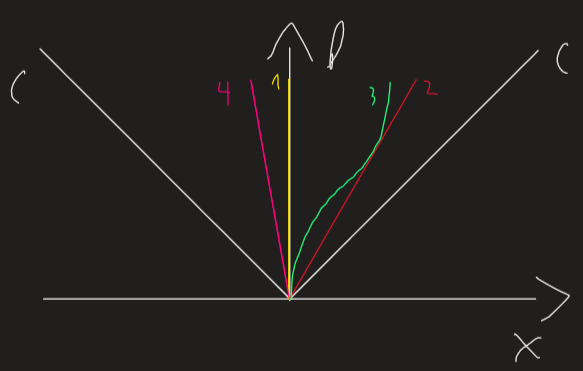
\includegraphics[scale = .5]{figures/4.2.2.png}
    \caption{Worldlines from the perspective of the first spaceship}
    \label{fig: Perspective 1}
  \end{figure}
  
  From the perspective \ref{fig: Situation 2} of spaceship 2 both ship 1 and the space station will have constant velocity away from it and ship 3 will accelerate away and then towards it and away again. The time-space diagram will then be as seen in figure \ref{fig: Perspective 2}
  \begin{figure}[h!]
    \centering
    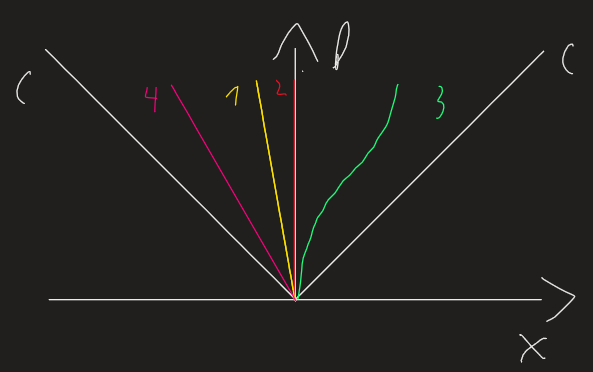
\includegraphics[scale = .5]{figures/4.2.3.png}
    \caption{Worldlines from the perspective of the second spaceship}
    \label{fig: Perspective 2}
  \end{figure}
  
  When looking at the diagram \ref{fig: Perspective 3} from the perspective of spaceship 3, all other ships will appear to accelerate and decelerate as itself will stay still in its own frame of reference. The time-space diagram will then be as seen in figure \ref{fig: Perspective 3} 
  \begin{figure}[h!]
    \centering
    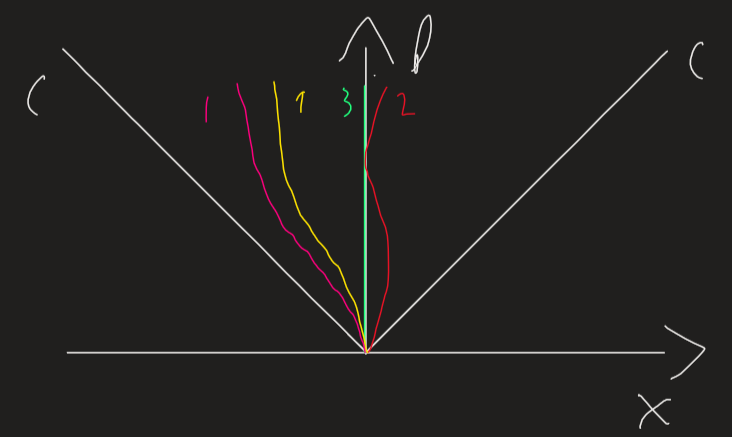
\includegraphics[scale = .5]{figures/4.5.png}
    \caption{Worldlines from the perspective of the third spaceship}
    \label{fig: Perspective 3}
  \end{figure}
  
  To see how much time has passed relative to each frame of reference we must draw time ticks on the time axis. This is the time the space stations perceives as it stands still. The blue arrows as seen in figure \ref{fig: Time Ticks}, is the time and space axis of the spaceship 2. We already know the space station measures 10 milliseconds when spaceship 2 measures only 8. We draw a line between them to show they happen simultaneously. The line is parallel with the space axis of ship 2. We found the lines spanning out $ x' $ and $ t' $ by using the angle $ α $ between the ship's position at event 2 and mirroring it around the line showing the worldline of a photon. 

  \begin{figure}[h!]
    \centering
    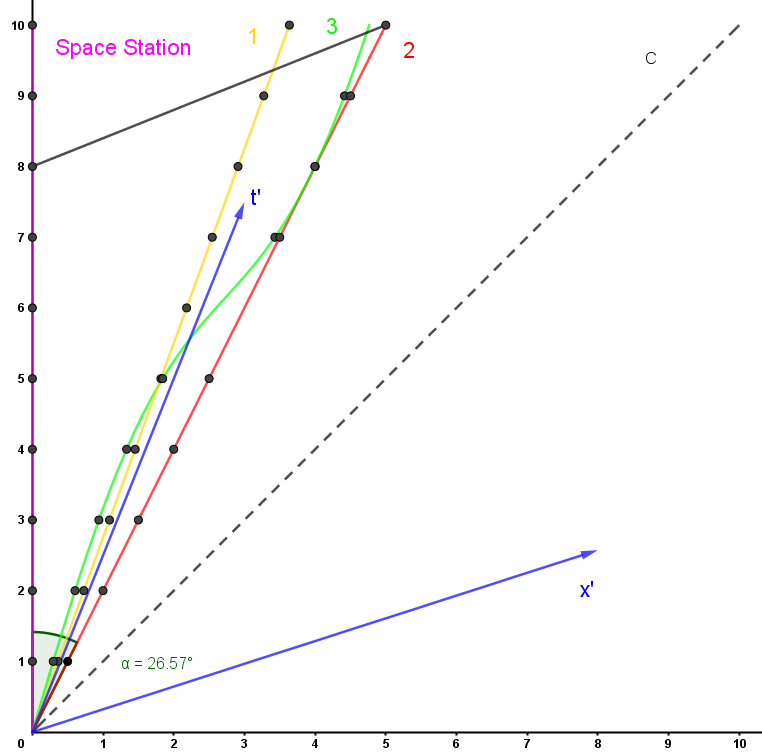
\includegraphics[scale = .5]{figures/4.10.png}
    \caption{Worldlines from the perspective of the station with time ticks}
    \label{fig: Time Ticks}
  \end{figure}
  
  \subsection{Conclusion} 
  
  As expected we get different worldlines depending on what perspective we use. When looking at the different time span measured by each observer its worth noticing how there is more spacing between each tick for ship 2's worldline. This is expected as we calculated in the previous exercise we found that $ Δt > Δt' $. 



\section{Exercise 7}

  \subsection{Introduction}

  \subsection{The Situation}

  \subsection{Method}

  \subsection{Conclusion} 

  \subsection{Specific Questions}



\section{Appendix} \label{sec: appendix}
\subsection{Exercise 1}
\subsubsection*{1.2.1}\label{1.2.1}
General equation for position
\[
r = r_0 + vt + \frac{1}{2} a^{2}
\]
The following are the positions of the left most spaceship $ r_L $, observer M $ r_M $ and the light beam emitted from the left most spaceship $ r_A $ in the reference frame of the planet.
\[
r_L = vt
\]
\[
r_M = \frac{L}{2} + vt
\]
\[
r_A = t
\]
\subsubsection*{1.2.2}\label{1.2.2}
The time it takes the laser to cross observer M is the time when the position of the laser is equal to the position of the observer M
\[
r_A = r_M
\]
\[
t = \frac{L}{2} + vt
\]
\[
t = \frac{L / 2}{1 - v}
\]  
Naturally it follows that $ t_M - t_A = t $ as derived above
\[
t_M - t_A = \frac{L / 2}{1 - v}
\]
\[
t_A = t_M - \frac{L / 2}{1 - v}
\]


\subsubsection*{1.2.3}\label{1.2.3}
\[
r_C = L - t
\]
Solving the following equation for $ t $
\[
r_M = r_C
\]
\[
\frac{L}{2} + vt = L - t
\]
\[
vt = \frac{L}{2} - t
\]
\[
t = \frac{L / 2}{v + 1}
\]
This is the time the beam uses to reach the spaceship. Naturally it follows that the time it takes to reach the observer is the time its shot out minus the time it hits the spaceship
\[
t_C - t_M = \frac{L / 2}{v + 1}
\]  
\[
t_C = t_M + \frac{L / 2}{v + 1}
\]
\\
\subsubsection*{1.2.4}\label{1.2.4}
We begin by calculating the time the laser reaches the opposite spaceship
\[
Δt =  t_C - t_A = \frac{L / 2}{v +1} + t_M - \left( t_M - \frac{L / 2}{1 - v} \right) 
\]
\[
Δt = \frac{L}{1 - v^{2}}
\]
From the perspective of the spaceship we don't need to take into the account the velocities of the spaceships. The time between the left most ship shooting and itself being shot will be the time it takes the light to travel the distance L as both ship shoots at the same time
\[
Δt': = L - t = 0
\]
\[
Δt' = L
\]


\subsection{Exercise 7}



\subsection{Other derivations}
\subsubsection*{1.1.2}\label{o: 1.1.2}
The time each laser uses to reach the observer $ M $ from the planets reference point. The position of the left most laser is $ r_L $, the observer $ r_M $  and the right most laser $ r_R $ is the following
\[
r_L = t
\]
\[
r_M = \frac{L}{2} + vt
\]
\[
r_R = -t
\]
Assuming the lasers are shot at the same time
\[
r_L = r_M
\]
\[
t = \frac{L}{2} + vt
\]
\[
t = \frac{L / 2}{1 - v}
\]
Doing the same for the right most laser
\[
r_R = r_M
\]
\[
-t = \frac{L}{2} + vt
\]
\[
t = \frac{L / 2}{1 + v}
\]
\subsubsection*{1.1.4}\label{o: 1.1.4}
These calculations are only meant to find the time it takes each beam to hit the opposing spaceship from the observer $ M $, not what the actual time it hits it.
We begin by solving when the position of the laser is equal to the position of the opposing ship. 
\[
t_C:= vt = -t + \frac{L}{2}
\]
\[
t_C = \frac{L/ 2}{1 + v}
\]
\[
t_D:= t = L + vt
\]
\[
t_D = \frac{L / 2}{1 - v}
\]

\section*{ACKNOWLEDGMENTS}

\section*{References} \label{sec: references}
\begin{enumerate}
  \item Refferer til forelesning notater 2a og b
  \item Reffere til notatene for bilde \label{ref: Example worldline}
\end{enumerate}


\end{document}